\documentclass[tikz]{standalone}
\usetikzlibrary{positioning}

% newcommands.tex

\newcommand{\enq}{\texttt{enq}}
\newcommand{\deq}{\texttt{deq}}
\newcommand{\pput}{\texttt{PUT}}
\newcommand{\get}{\texttt{GET}}
\newcommand{\vs}{\texttt{vis}}
\newcommand{\so}{\texttt{so}}
\newcommand{\arb}{\texttt{ar}}
\newcommand{\rf}{\texttt{rf}}

% example
\newcommand{\po}[2]{\draw [->, thick] (#1) to node[above] {\Large{\so}} (#2);}
\newcommand{\pva}[2]{\draw [->, thick] (#1) to node[above] {$\Large{\so},\Large{\vs},\Large{\arb}$} (#2);}
\newcommand{\pbva}[2]{\draw [->, thick] (#1) to node[above] {$\Large{\so}$} node[below] {$\Large{\vs},\Large{\arb}$} (#2);}
\newcommand{\pv}[2]{\draw [->, thick] (#1) to node[above] {\Large{\so}} node[below] {\Large{\vs}} (#2);}
\newcommand{\evis}[2]{\draw [->, thick] (#1) to node[above, sloped, near end] {\Large{\vs}} (#2);}
\newcommand{\mvis}[2]{\draw [->, thick] (#1) to node[above, sloped] {\Large{\vs}} (#2);}
\newcommand{\ar}[2]{\draw [->, thick, allow upside down] (#1) to node[above, sloped] {\Large{\arb}} (#2);}
\newcommand{\va}[2]{\draw [->, thick, allow upside down] (#1) to node[above, sloped] {$\Large{\vs},\Large{\arb}$} (#2);}
\newcommand{\vab}[2]{\draw [->, thick, allow upside down] (#1) to node[below, sloped, near end] {$\Large{\vs},\Large{\arb}$} (#2);}
\newcommand{\vae}[2]{\draw [->, thick, allow upside down] (#1) to node[above, sloped, near end] {$\Large{\vs},\Large{\arb}$} (#2);}
\newcommand{\vas}[2]{\draw [->, thick, allow upside down] (#1) to node[sloped, near start, above] {$\Large{\vs},\Large{\arb}$} (#2);}

% serialization
\newcommand{\scc}[2]{\draw [->, very thick] (#1) to (#2);}
\newcommand{\rva}[2]{\draw [->, thick, allow upside down] (#1) to node[above, sloped] {$\Large{\rf},\Large{\vs},\Large{\arb}$} (#2);}
\newcommand{\rvb}[2]{\draw [->, thick, allow upside down] (#1) to node[below, sloped] {$\Large{\rf},\Large{\vs},\Large{\arb}$} (#2);}


\renewcommand{\va}[2]{\draw [->, thick] (#1) to node[above, sloped,pos=0.55] {$\Large{\vs},\Large{\arb}$} (#2);}
\renewcommand{\vab}[2]{\draw [->, thick] (#1) to node[above, sloped,pos=0.75] {$\Large{\arb}$} (#2);}

\newcommand{\visar}[2]{\draw [->, thick] (#1) to [out=340,in=200] node[above, pos = 0.6] {$\Large{\vs},\Large{\arb}$} (#2);}
%\newcommand{\visar}[2]{\draw [->, thick] (#1) to [out=20,in=160] node[above, pos = 0.8] {$\Large{\vs},\Large{\arb}$} (#2);}

\begin{document}
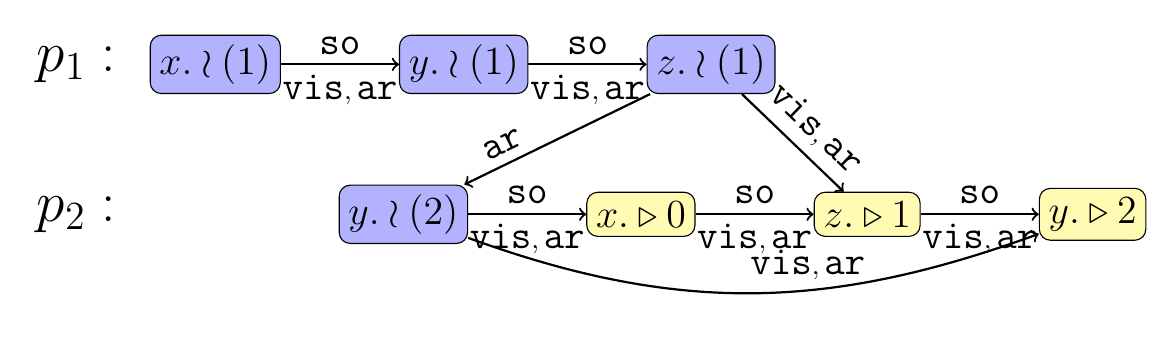
\begin{tikzpicture}
\tikzset{
  wop/.style = {rectangle, rounded corners, fill = blue!30, draw, font = \Large},
  rop/.style = {rectangle, rounded corners, fill = yellow!30, draw, font = \Large}, process/.style = {font = \huge},
  %po/.style = {->, very thick},
  rw/.style = {->, shorten >= 3pt, very thick, dashed},
  %vis/.style = {->, shorten >= 3pt, very thick, dashed}
}

  \node (p1) [process] {$p_1:$};
  \node (wx1) [wop, right = 0.3cm of p1] {$x.\wr(1)$};
  \node (wy1) [wop, right = 1.5cm of wx1] {$y.\wr(1)$};
  \node (wz1) [wop, right = 1.5cm of wy1] {$z.\wr(1)$};

  \node (p2) [process, below = 1.2cm of p1] {$p_2:$};
  \node (wy2) [wop, right = 2.7cm of p2] {$y.\wr(2)$};
  \node (rx0) [rop, right = 1.5cm of wy2] {$x.\rd\triangleright0$};
  \node (rz1) [rop, right = 1.5cm of rx0] {$z.\rd\triangleright1$};
  \node (ry2) [rop, right = 1.5cm of rz1] {$y.\rd\triangleright2$};

  \pbva{wx1}{wy1};
  \pbva{wy1}{wz1};

  \pbva{wy2}{rx0};
  \pbva{rx0}{rz1};
  \pbva{rz1}{ry2};

  \va{wz1}{rz1};

  \vab{wz1}{wy2};
  \visar{wy2}{ry2};
  
\end{tikzpicture}
\end{document}
